\documentclass[12pt]{article}
\usepackage{amsmath}
\usepackage{amsfonts}
\usepackage{amssymb}
\usepackage{graphicx}
\usepackage{hyperref}
\usepackage{lipsum}
\usepackage{tikz}
\usetikzlibrary{matrix, calc}

\title{\textbf{Efficient Eigenvalue Determination in Complex Matrices through the QR Iterative Method}}
\author{Akshara Sarma Chennubhatla \\EE24BTECH11003\\ Department of Electrical Engineering \\ IIT Hyderabad}
\date{\today}

\begin{document}

\maketitle

\begin{abstract}
This report outlines the calculation of eigenvalues of a complex matrix using the QR algorithm, implemented through Householder transformations and Givens rotations. Additionally, strategies for improving convergence, such as the Rayleigh quotient shift, are discussed. Challenges posed by Jordan blocks are addressed, and a comparison of the QR algorithm with other eigenvalue computation methods, focusing on time complexity, accuracy, and suitability for different types of matrices, is provided.
\end{abstract}

\section{Introduction}
Eigenvalues are scalar values associated with a square matrix \(A\) that satisfy:

\[
A \mathbf{v} = \lambda \mathbf{v},
\]

where \(\mathbf{v}\) is a non-zero eigenvector. Eigenvalues are fundamental to many scientific and engineering applications, including vibration analysis, quantum mechanics, and dimensionality reduction techniques like Principal Component Analysis (PCA).

The QR algorithm is a robust iterative method for eigenvalue computation. It iteratively transforms a matrix into an upper triangular form, from which the eigenvalues can be read directly from the diagonal. This report explores the QR algorithm's implementation, including enhancements for faster convergence and handling special cases such as Jordan blocks.

\section{QR Algorithm Overview}
The QR algorithm decomposes a matrix \(A\) into the product of an orthogonal matrix \(Q\) and an upper triangular matrix \(R\), such that:

\[
A = QR.
\]

The matrix is then updated iteratively as:

\[
A_{\text{new}} = RQ.
\]

This process is repeated until \(A\) converges to an upper triangular form. To accelerate convergence and ensure numerical stability, the matrix is first reduced to Hessenberg form.

\subsection{Enhancing Convergence with the Rayleigh Quotient Shift}
To improve convergence, the QR algorithm can be enhanced by applying the **Rayleigh quotient shift**. This technique selects a shift \(\sigma\) close to an eigenvalue of \(A\), effectively speeding up convergence and reducing the number of iterations.

\subsubsection{Implementation}
The Rayleigh quotient shift involves the following steps:
\begin{enumerate}
    \item Compute the shift:
    \[
    \sigma = A_{n,n},
    \]
    where \(A_{n,n}\) is the bottom-right entry of the current matrix \(A\), approximating an eigenvalue.
    \item Update the matrix by subtracting the shift:
    \[
    A - \sigma I,
    \]
    where \(I\) is the identity matrix.
    \item Perform QR decomposition on the shifted matrix:
    \[
    A - \sigma I = QR.
    \]
    \item Recalculate \(A\) by applying the inverse shift:
    \[
    A_{\text{new}} = RQ + \sigma I.
    \]
\end{enumerate}

This shifting mechanism "pushes" the matrix closer to its triangular form, accelerating convergence.

\subsubsection{Advantages of the Rayleigh Quotient Shift}
The shift offers the following benefits:
\begin{itemize}
    \item \textbf{Faster Convergence:} Reduces the number of iterations needed for the matrix to converge, particularly for matrices with closely spaced eigenvalues.
    \item \textbf{Numerical Stability:} Mitigates rounding errors by maintaining well-conditioned matrices during iterations.
    \item \textbf{Dynamic Adaptation:} The shift updates dynamically based on the current matrix, enhancing accuracy.
\end{itemize}

The Rayleigh quotient shift is particularly effective for symmetric matrices, where it achieves cubic convergence.

\section{Matrix Reduction to Hessenberg Form}
Reducing a matrix to Hessenberg form simplifies subsequent QR iterations while preserving eigenvalues. A Hessenberg matrix \(H\) has non-zero entries only on the main diagonal and the first sub-diagonal.


\[
H = 
\begin{bmatrix}
h_{11} & h_{12} & h_{13} & \cdots & h_{1n} \\
h_{21} & h_{22} & h_{23} & \cdots & h_{2n} \\
0      & h_{32} & h_{33} & \cdots & h_{3n} \\
\vdots & \ddots & \ddots & \ddots & \vdots \\
0      & \cdots & 0      & h_{n-1,n-1} & h_{n-1,n} \\
0      & \cdots & \cdots & 0          & h_{nn} \\
\end{bmatrix}.
\]

The zeros below the subdiagonal are introduced using Householder transformations, which are applied iteratively to eliminate elements in each column below the diagonal.


\subsection{Householder Transformations}
The Householder transformation is a method to zero out elements below the diagonal in a column vector. For complex matrices, each element of the matrix is a complex number, and the transformation proceeds as follows.

\subsubsection{Householder Transformation for Complex Matrices}
The goal of the Householder transformation is to eliminate the sub-diagonal elements in the matrix and reduce it to Hessenberg form. The process for complex matrices is as follows:

1. **Select a Subvector \( x \):**
   We begin by selecting the subvector \( x \) from the first column of the matrix \( A \), starting from the element just below the diagonal, i.e., \( A_{2,1} \), down to \( A_{n,1} \). This is represented as:

   \[
   x = \begin{bmatrix}
   A_{2,1} \\
   A_{3,1} \\
   \vdots \\
   A_{n,1}
   \end{bmatrix}.
   \]

   Each element in \( x \) is a complex number of the form \( A_{i,1} = a_{i,1} + ib_{i,1} \), where \( a_{i,1} \) and \( b_{i,1} \) are the real and imaginary parts, respectively.

2. **Define the Target Vector:**
   The goal is to transform \( x \) into a new vector \( y \) where only the first element is non-zero, and all the other elements are zero. First, compute the norm of \( x \):

   \[
   \| x \| = \sqrt{|A_{2,1}|^2 + |A_{3,1}|^2 + \dots + |A_{n,1}|^2},
   \]

   where \( |z| = \sqrt{a^2 + b^2} \) for a complex number \( z = a + ib \). Then define the target vector \( y \) as:

   \[
   y = \pm \| x \| e_1,
   \]

   where \( e_1 = \begin{bmatrix} 1 \\ 0 \\ \vdots \\ 0 \end{bmatrix} \) is the first standard basis vector, and the sign is chosen to avoid numerical cancellation.

3. **Construct the Householder Vector \( v \):**
   To generate a reflection that transforms \( x \) to \( y \), the Householder vector \( v \) is defined as:

   \[
   v = x - \text{sign}(x_1) \| x \| e_1.
   \]

   The sign of the first element \( x_1 \) is crucial. In the case of a complex number, \( \text{sign}(x_1) \) is defined as:

   \[
   \text{sign}(x_1) = \frac{x_1}{|x_1|},
   \]

   where \( x_1 \) is the first element of the vector \( x \), and \( |x_1| \) is its modulus (i.e., \( |x_1| = \sqrt{a_1^2 + b_1^2} \) for a complex number \( x_1 = a_1 + ib_1 \)).

   After defining \( v \), it is normalized to a unit vector:

   \[
   v \leftarrow \frac{v}{\|v\|}.
   \]

4. **Construct the Householder Matrix \( H_k \):**
   The Householder matrix \( H_k \) is constructed as:

   \[
   H_k = I - 2 \frac{v v^*}{v^* v},
   \]

   where \( v^* \) denotes the complex conjugate transpose of \( v \), and \( I \) is the identity matrix. This matrix \( H_k \) will zero out the sub-diagonal elements of the first column when applied to \( A \).

5. **Apply the Householder Transformation:**
   The matrix \( H_k \) is applied to \( A \) as:

   \[
   A' = H_k A H_k^*,
   \]

   where \( H_k^* \) is the conjugate transpose of \( H_k \). This will reduce the matrix to Hessenberg form by eliminating the sub-diagonal elements of the first column.

6. **Repeat for Subsequent Columns:**
   The above steps are repeated for each subsequent column of the matrix until the matrix is in Hessenberg form.

This Householder transformation approach ensures that the matrix is gradually transformed to a Hessenberg form, where all elements below the first sub-diagonal are zero.

\subsection{Givens Rotations}
Once the matrix is in Hessenberg form, QR decomposition is performed using Givens rotations. These rotations zero out specific off-diagonal elements while preserving the Hessenberg structure.


\begin{center}
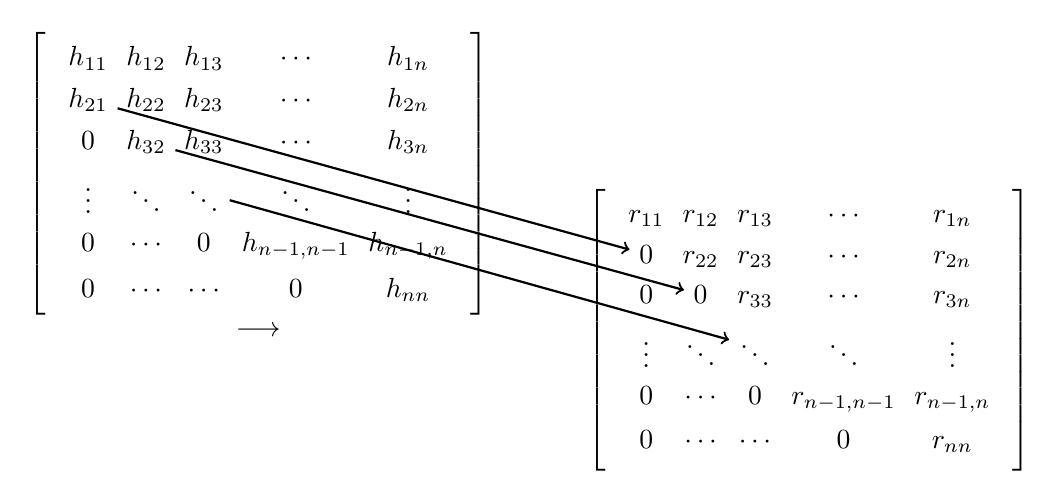
\begin{tikzpicture}
  % Original Hessenberg Matrix
  \matrix[matrix of math nodes, left delimiter={[}, right delimiter={]}] (hessenberg) {
    h_{11} & h_{12} & h_{13} & \cdots & h_{1n} \\
    h_{21} & h_{22} & h_{23} & \cdots & h_{2n} \\
    0      & h_{32} & h_{33} & \cdots & h_{3n} \\
    \vdots & \ddots & \ddots & \ddots & \vdots \\
    0      & \cdots & 0      & h_{n-1,n-1} & h_{n-1,n} \\
    0      & \cdots & \cdots & 0          & h_{nn} \\
  };

  % Arrow indicating Givens rotation
  \node[above of=hessenberg, yshift=-3cm] (arrow) {\(\longrightarrow\)};
  
  % Upper Triangular Matrix after QR
  \matrix[matrix of math nodes, left delimiter={[}, right delimiter={]}, right of=arrow, xshift=6cm] (upper) {
    r_{11} & r_{12} & r_{13} & \cdots & r_{1n} \\
    0      & r_{22} & r_{23} & \cdots & r_{2n} \\
    0      & 0      & r_{33} & \cdots & r_{3n} \\
    \vdots & \ddots & \ddots & \ddots & \vdots \\
    0      & \cdots & 0      & r_{n-1,n-1} & r_{n-1,n} \\
    0      & \cdots & \cdots & 0          & r_{nn} \\
  };

  % Arrows to show step-by-step elimination
  \draw[->, thick] (hessenberg-2-1) -- (upper-2-1);
  \draw[->, thick] (hessenberg-3-2) -- (upper-3-2);
  \draw[->, thick] (hessenberg-4-3) -- (upper-4-3);
\end{tikzpicture}
\end{center}

Each Givens rotation zeros out a specific subdiagonal element, progressively transforming the Hessenberg matrix into an upper triangular matrix.


\subsubsection{Definition of Givens Rotations}
A Givens rotation is a plane rotation that operates on any arbitrary \(2 \times 2\) block in a matrix. The rotation is represented as:

\[
G(i, j, \theta) =
\begin{bmatrix}
1 &\cdots& 0& \cdots& 0 &\cdots& 0 &\cdots& 0 \\
\vdots &\ddots& \vdots && \vdots && \vdots&& \vdots \\
0 &\cdots& c & \cdots& s &\cdots & 0&\cdots& 0 \\
\vdots && \vdots &\ddots& \vdots && \vdots&& \vdots \\
0 &\cdots& -\bar{s}& \cdots& \bar{c} &\cdots& 0 &\cdots& 0\\
\vdots && \vdots && \vdots &\ddots& \vdots&& \vdots \\
0 &\cdots& 0 & \cdots& 0 &\cdots & 1&\cdots& 0\\
\vdots && \vdots && \vdots && \vdots &\ddots& \vdots \\
0 &\cdots& 0 & \cdots& 0 &\cdots &0&\cdots& 1\\

\end{bmatrix},
\]

where \( c = \cos(\theta) \) and \( s = \sin(\theta) \), and the matrix acts on a general \( 2 \times 2 \) block of the form \( (i, j) \), with all the other elements of the identity matrix being zero. Here \( i \) and \( j \) represent the row and column indices of the block being rotated.

The entries outside the \( 2 \times 2 \) block are identity entries. The matrix is identity everywhere except for the \( 2 \times 2 \) block in positions \( (i,i), (i+1,i), (i,i+1), (i+1,i+1) \).


\subsection{Steps of the Givens Rotation Algorithm}

The QR decomposition using Givens rotations proceeds as follows:

\subsubsection{Step 1: Hessenberg Form}
Before applying Givens rotations, the matrix must be reduced to Hessenberg form using Householder transformations (as described earlier). A matrix \( H \) in Hessenberg form has non-zero entries only on the main diagonal and the first sub-diagonal.

\subsubsection{Step 2: Initialize the Matrix}
Given a Hessenberg matrix \( H \), we aim to decompose it into the product of an orthogonal matrix \( Q \) and an upper triangular matrix \( R \):

\[
H = Q R,
\]

where \( Q \) is an orthogonal matrix (i.e., \( Q^T Q = I \)) and \( R \) is upper triangular. To achieve this, we perform Givens rotations.

\subsubsection{Step 3: Apply Givens Rotations to Zero Out Subdiagonal Elements}
At each iteration, we focus on a pair of adjacent elements in the matrix \( H \), specifically \( H(i, j) \) and \( H(i+1, j) \), and apply a Givens rotation to eliminate the subdiagonal element \( H(i+1, j) \).

A Givens rotation matrix \( G(i, j, \theta) \) is designed to zero out the element \( H(i+1, j) \) while leaving the rest of the matrix unchanged. The angle \( \theta \) is chosen such that the new elements become:

\[
H(i, j) \rightarrow r, \quad H(i+1, j) \rightarrow 0,
\]

where \( r \) is the norm of the 2-by-2 block formed by \( H(i, j) \) and \( H(i+1, j) \), computed as:

\[
r = \sqrt{H(i, j)^2 + H(i+1, j)^2}.
\]

The values of the cosine \( c \) and sine \( s \) of the Givens rotation are then:

\[
c = \frac{H(i, j)}{r}, \quad s = \frac{H(i+1, j)}{r}.
\]

This ensures that the following transformation occurs:

\[
\begin{bmatrix} 
H(i, j) & H(i+1, j) \\
H(i, j+1) & H(i+1, j+1)
\end{bmatrix}
\longrightarrow
\begin{bmatrix}
r & 0 \\
0 & H(i+1, j+1)
\end{bmatrix}.
\]

The Givens rotation \( G(i, j, \theta) \) is applied to the matrix \( H \) as follows:

\[
H' = G(i, j, \theta) H,
\]

which zeroes out the element \( H(i+1, j) \) and updates the matrix to \( H' \).

\subsubsection{Step 4: Update the Matrix}
The updated matrix \( H' \) after applying the Givens rotation is an intermediate matrix where one subdiagonal element is zeroed out. The process is then repeated for the next pair of elements in the matrix.

\subsubsection{Step 5: Continue Until All Subdiagonal Elements are Zero}
This process is repeated for all subdiagonal elements of the matrix. Each time, a Givens rotation is applied to a \( 2 \times 2 \) block in the matrix, progressively eliminating all subdiagonal elements, resulting in a matrix \( R \) that is upper triangular.

\subsubsection{Step 6: Construct the Matrix \( Q \) and Matrix \( R \)}
For each Givens rotation applied, we construct an orthogonal matrix \( Q \) and \( R \). Initially, \( Q \) is the identity matrix and \( R \) is the matrix \( H \), and at each step, we update \( R \) by multiplying it with the corresponding Givens rotation matrix from the left and update \( Q \) by multiplying with the corresponding transpose of the Givens rotation matrix from the right:

\[
R' = G(i, j, \theta) R
\] 
\[ 
Q' = Q G^{T}(i, j, \theta).
\]

At the end of the process, the matrix \( Q \) will be the orthogonal matrix that satisfies the QR decomposition:

\[
H = Q R.
\]

\subsection{Summary of the Givens Rotation Algorithm Steps:}
\begin{enumerate}
    \item Reduce the matrix to Hessenberg form using Householder transformations.
    \item For each column, apply a Givens rotation to zero out the subdiagonal element.
    \item Update the matrix at each step, and repeat for the next subdiagonal element.
    \item After completing the iterations, the matrix \( R \) will be upper triangular, and the matrix \( Q \) will be orthogonal.
\end{enumerate}

\section{Handling Jordan Blocks}
Jordan blocks pose challenges in eigenvalue computation because the matrix cannot be diagonalized. A Jordan block for eigenvalue \(\lambda\) appears as:

\[
\begin{bmatrix}
a & b \\
c & d
\end{bmatrix}
\]

where a and b are the diagonal elements and c is a non zero sub-diagonal element.\\
To handle Jordan blocks, the QR algorithm implemented here solves for the eigenvalues directly using the characteristic polynomial of the block. For a \(2 \times 2\) Jordan block, the eigenvalues are roots of:

\[
\lambda^2 - (\text{trace})\lambda + \det = 0.
\]

For larger number of Jordan blocks, the process involves recursive computation of characteristic polynomials. Explicitly addressing Jordan blocks ensures accurate eigenvalue determination even when the matrix is not diagonalizable.

\section{Time Complexity}
The time complexity of the QR algorithm with Givens rotations is primarily determined by the matrix multiplication and decomposition steps. Each iteration involves multiplying matrices and performing Givens rotations, each of which takes \( O(n^3) \) time. Thus, the overall time complexity for \( m \) iterations is:
\[
O(m \cdot n^3)
\]
where \( n \) is the size of the matrix and \( m \) is the number of iterations required for convergence. In practice, the QR algorithm converges within \( n^2 \) iterations for matrices with distinct eigenvalues.

\section{Memory Complexity}
The memory complexity is driven by the storage requirements for the input matrix, the \( Q \) and \( R \) matrices, and any intermediate matrices used during the algorithm. Each matrix requires \( O(n^2) \) memory, leading to an overall space complexity of:
\[
O(n^2)
\]

\section{Advantages of the QR Algorithm}
The QR algorithm, implemented in the provided code, exhibits several advantages due to its design and enhancements:  

\begin{itemize}
    \item \textbf{Efficient Convergence Handling:} The algorithm terminates iterations as soon as the matrix converges to an upper triangular form and runs for a maximum of 1000 iterations if not. This dynamic stopping criterion ensures computational efficiency, avoiding unnecessary iterations.
    \item \textbf{Accelerated Convergence with Shifts:} By incorporating the Rayleigh quotient shift, the algorithm speeds up convergence significantly. This is particularly beneficial for matrices with closely spaced or complex eigenvalues, reducing the total number of iterations.
    \item \textbf{Numerical Stability:} The use of orthogonal transformations (Householder transformations and Givens rotations) minimizes rounding errors, making the algorithm reliable even for large or ill-conditioned matrices.
    \item \textbf{General Applicability:} The algorithm is suitable for both symmetric and non-symmetric matrices, as well as for real and complex matrices.
    \item \textbf{Robustness in Handling Special Cases:} The implementation effectively handles Jordan blocks by solving characteristic polynomials for \(2 \times 2\) submatrices, ensuring correct eigenvalue determination even for non-diagonalizable matrices.
    \item \textbf{Efficiency for Dense Matrices:} The method is efficient for dense matrices, where most elements are non-zero, due to the structured use of Hessenberg reduction and QR decomposition.
\end{itemize}

\section{Comparison with Other Methods}
The QR algorithm, as implemented, offers several advantages over other eigenvalue computation methods due to its efficiency, accuracy, and robustness. Below is a comparison:  

\begin{itemize}
    \item \textbf{Power Iteration:}  
    - The power iteration method is fast for finding the dominant eigenvalue but fails to compute all eigenvalues.  
    - Convergence is slow, especially for matrices with eigenvalues of similar magnitudes.  
    - Unlike power iteration, the QR algorithm in this implementation computes all eigenvalues efficiently, leveraging shifts to improve convergence.  

    \item \textbf{Jacobi Method:}  
    - While accurate for symmetric matrices, the Jacobi method is computationally expensive for general matrices.  
    - The QR algorithm, with its Hessenberg reduction and Givens rotations, outperforms Jacobi in handling non-symmetric or complex matrices.  

    \item \textbf{Divide and Conquer:}  
    - This method is faster for large matrices but requires significantly more memory and is more complex to implement.  
    - In contrast, the QR algorithm balances memory usage (\(O(n^2)\)) with computational efficiency, making it more suitable for medium-sized dense matrices.  

    \item \textbf{Special Case Handling:}  
    - Methods like power iteration and Jacobi struggle with Jordan blocks or closely spaced eigenvalues.  
    - The QR algorithm addresses these challenges robustly by leveraging dynamic convergence detection and the Rayleigh quotient shift.  
\end{itemize}

\section{Convergence Rate}
The convergence of the QR algorithm is accelerated in the implemented version by using the Rayleigh quotient shift. Key points include:  

\begin{itemize}
    \item \textbf{Quadratic Convergence:} For matrices with distinct eigenvalues, the QR algorithm exhibits quadratic convergence, where the error decreases significantly with each iteration.  
    \item \textbf{Cubic Convergence with Shifts:} The use of the Rayleigh quotient shift often results in cubic convergence for symmetric matrices or matrices with eigenvalues close in magnitude. This significantly reduces the number of iterations required.  
    \item \textbf{Dynamic Stopping Criterion:} The algorithm stops as soon as convergence to an upper triangular form is achieved, further optimizing the computation time.  
\end{itemize}

For matrices with Jordan blocks or multiple eigenvalues, the algorithm adapts by handling \(2 \times 2\) submatrices explicitly, ensuring stability and correctness.  

\section{When This Method Works Better}
The QR algorithm, as implemented in this report, is particularly advantageous in the following scenarios:  

\begin{center}
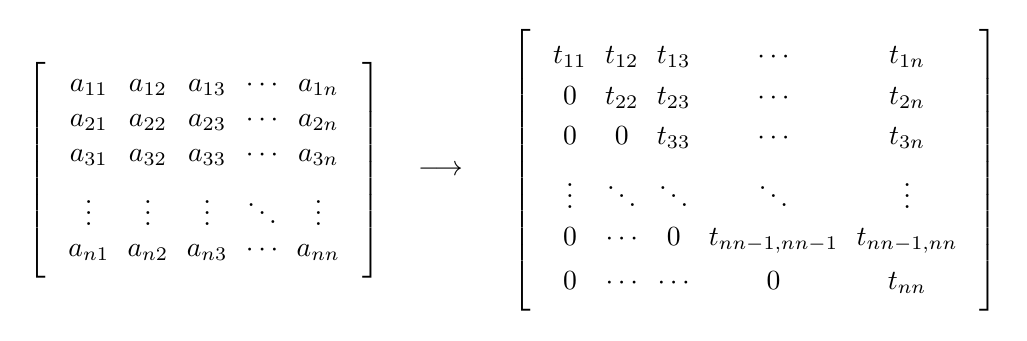
\begin{tikzpicture}
  % Initial General Matrix
  \matrix[matrix of math nodes, left delimiter={[}, right delimiter={]}] (general) {
    a_{11} & a_{12} & a_{13} & \cdots & a_{1n} \\
    a_{21} & a_{22} & a_{23} & \cdots & a_{2n} \\
    a_{31} & a_{32} & a_{33} & \cdots & a_{3n} \\
    \vdots & \vdots & \vdots & \ddots & \vdots \\
    a_{n1} & a_{n2} & a_{n3} & \cdots & a_{nn} \\
  };

  % Arrow to show progression
  \node[above of=general, yshift= -1cm,xshift = 3cm] (arrow2) {\(\longrightarrow\)};
  
  % Final Upper Triangular Matrix
  \matrix[matrix of math nodes, left delimiter={[}, right delimiter={]}, right of=arrow2, xshift=3cm] (triangular) {
    t_{11} & t_{12} & t_{13} & \cdots & t_{1n} \\
    0      & t_{22} & t_{23} & \cdots & t_{2n} \\
    0      & 0      & t_{33} & \cdots & t_{3n} \\
    \vdots & \ddots & \ddots & \ddots & \vdots \\
    0      & \cdots & 0      & t_{nn-1,nn-1} & t_{nn-1,nn} \\
    0      & \cdots & \cdots & 0          & t_{nn} \\
  };
\end{tikzpicture}
\end{center}

By leveraging Hessenberg reduction and iterative shifts, the algorithm converges to an upper triangular form efficiently.


\begin{itemize}
    \item \textbf{Dense Matrices:} The combination of Hessenberg reduction, Givens rotations, and shifts makes the QR algorithm highly efficient for dense matrices where most elements are non-zero.  
    \item \textbf{Complex Eigenvalues:} By using shifts, the algorithm converges quickly even for complex matrices with eigenvalues close in magnitude.  
    \item \textbf{Non-Diagonalizable Matrices:} The implementation's ability to handle Jordan blocks ensures robustness for matrices that cannot be diagonalized.  
    \item \textbf{Numerical Stability:} The orthogonal transformations used in the QR algorithm minimize rounding errors, making it reliable for applications requiring high precision.  
    \item \textbf{Medium-Sized Matrices:} While scalable, the QR algorithm strikes an ideal balance of memory usage and computational complexity for medium-sized matrices (\(n \leq 1000\)).  
\end{itemize}

\section{Code Reference}
This is my C code implementation of solving the Eigenvalue problem using the algorithm explained above. This is the link to my GitHub repository.\\
\url{https://github.com/Akshara778/EE1030/tree/main/Software_assignment}

\begin{thebibliography}{99}

\bibitem{ref1} Arbenz, P. (n.d.). \textit{Eigenvalue Problems and QR Algorithm}. Retrieved from \url{https://people.inf.ethz.ch/arbenz/ewp/Lnotes/chapter4.pdf}

\bibitem{ref2} \textit{QR Algorithm for Eigenvalues}. (2015, March 23). Retrieved from \url{https://www.youtube.com/watch?v=PFDu9oVAE-g&pp=ygUKZWlnZW52YWx1ZQ%3D%3D}

\bibitem{ref3} \textit{QR Decomposition and Eigenvalues}. (2020, October 22). Retrieved from \url{https://www.youtube.com/watch?v=moTxjgVEBfA&t=550s&pp=ygUGZ2l2ZW5z}

\bibitem{ref4} Wikipedia contributors. (n.d.). \textit{QR Algorithm}. Wikipedia. Retrieved from \url{https://en.wikipedia.org/wiki/QR_algorithm}

\bibitem{ref5} EE1010 Course Notes, \textit{Lecture Notes on Eigenvalue Computation}, Retrieved from the course repository.

\end{thebibliography}

\end{document}
